\documentclass[aspectratio=169]{beamer}

\usepackage{tikz}
\usetikzlibrary{calc,shapes.geometric,positioning,arrows.meta}

\usepackage{bbm}
\usepackage{booktabs}
\usepackage{amsmath}

\definecolor{huaweired}{RGB}{206,14,45}
\definecolor{titledred}{RGB}{153,0,0}
\definecolor{bannergray}{RGB}{128,128,128}

\setbeamercolor{frametitle}{fg=titledred}
\setbeamerfont{frametitle}{series=\bfseries,size=\LARGE}
\setbeamertemplate{navigation symbols}{}
\setbeamertemplate{itemize item}{\color{black}$\bullet$}
\setbeamertemplate{itemize subitem}{\color{black}--}

\newlength{\footerlineleft}
\newlength{\footerlineright}
\newlength{\footerlinebottomgap}

\setlength{\footerlineleft}{0.7em}       
\setlength{\footerlineright}{0.7em}      
\setlength{\footerlinebottomgap}{0.14em}  

\setbeamertemplate{footline}{
  \leavevmode
  \vbox{
    \hbox to \paperwidth{
      \hspace*{\footerlineleft}
      {\color{titledred}
        \rule{
          \dimexpr\paperwidth
          -\footerlineleft
          -\footerlineright\relax
        }{0.4pt}
      }
      \hspace*{\footerlineright}
    }
    \vskip\footerlinebottomgap

    \hbox{
      \begin{beamercolorbox}[
        wd=\paperwidth,
        ht=2.6ex,
        dp=1.6ex,
        leftskip=1.5em,
        rightskip=1.5em
      ]{footline}
        \footnotesize
        HUAWEI TECHNOLOGIES CO., LTD.
        \hfill
        Huawei Confidential
        \hfill
        Page~\insertframenumber
        \hspace{2em}
        \raisebox{-0.6ex}{
          \includegraphics[height=2.6ex]{huawei_logo.pdf}
        }
        \textbf{\footnotesize HUAWEI}
      \end{beamercolorbox}
    }
  }
}

\newcommand{\titlerule}{{\color{titledred}\hrule height 1.2pt}}


\newcommand{\HuaweiTitleSlide}[2]{%
{
\setbeamertemplate{footline}{}
\begin{frame}[plain]
\begin{tikzpicture}[remember picture,overlay]
  \fill[bannergray]
    (current page.west) ++(0,1.35)
    -- ++(11.4,0)
    -- ++(-0.85,-3.45)
    -- ($(current page.west)+(0,-2.1)$)
    -- cycle;

  \fill[huaweired]
    ($(current page.west)+(12.6,1.35)$)
    .. controls ($(current page.west)+(11.9,-0.6)$) ..
    ($(current page.west)+(11.05,-2.1)$)
    -- ($(current page.east)+(0,-2.1)$)
    -- ($(current page.east)+(0,1.35)$)
    -- cycle;

  \node[anchor=north east] at ($(current page.north east)+(-0.9,-0.9)$)
    {\large\bfseries Security Level: SECRET};

  \node[anchor=west, text=white] at ($(current page.west)+(0.9,0.55)$)
    {\resizebox{9.8cm}{!}{\Huge\bfseries #1}};

  \node[text=white] at ($(current page.center)+(-1.0,-1.35)$)
    {\large\bfseries NetMind Canada};

  \node[anchor=east, text=white] at ($(current page.east)+(-0.7,-1.45)$)
    {\normalsize www.huawei.com};

  \node at ($(current page.center)+(0,-2.5)$)
    {\large\bfseries Mohammad Hossein Moslemi (m84449988) / #2};

  \node[anchor=north west] at ($(current page.north west)+(0.9,-0.1)$)
    {\begin{tabular}{c}\includegraphics[width=1.5cm]{huawei_logo.pdf}\\[-1pt]{\large\bfseries HUAWEI}\end{tabular}};

\end{tikzpicture}
\end{frame}
}
}

\begin{document}

\HuaweiTitleSlide{Dynamic PUCT: Global Prior-Guided Test-Time Search}{}

\begin{frame}{Standard PUCT}
\vspace{-1em}
{\color{titledred}\hrule height 1.2pt}
\vspace{1.4em}

\begin{equation*}
\text{PUCT}(s) \;=\;
\underbrace{\frac{W(s)}{m_s}}_{\substack{\text{exploitation:}\\ \text{mean value of subtree}}}
\;+\;
c \cdot P(s \mid p) \cdot
\underbrace{\frac{\sqrt{m_p}}{1 + m_s}}_{\substack{\text{exploration:}\\ \text{favors rarely visited children}}}
\end{equation*}

\vspace{1em}
\begin{itemize}
  \item $W(s) = \sum_{y \in \mathcal{T}(s)} Q(y)$: accumulated value of the subtree rooted at $s$
  \item $m_s = |\mathcal{T}(s)|$: subtree size (used in place of visit count)
  \item $P(s \mid p) = \mathrm{softmax}\big(\{\, Q(s') \mid s' \in \mathcal{S}(p) \,\}\big)_s$: child prior
\end{itemize}


  \vspace{2em}
  \textbf{D-PUCT}$\rightarrow$
Stands for Dynamic-PUCT. Replace exploitation term by $\max_{s' \in \mathcal{T}Q(s')}$, and the $P(s|p)$ by the ``Global Node prior'' and ``Virtual Child''.
\end{frame}











\begin{frame}{Global Node Logit $L_D(s)$}
\vspace{0.8em}
{\color{titledred}\hrule height 1.2pt}
\vspace{1em}

All nodes in the search tree are stored in a flat dataset \(D\).
For every node \(s \in D\), we compute two dataset-level signals:

\vspace{-0.4em}
{\footnotesize
\begin{align}
  \text{Rank signal}
  &\;\longrightarrow\;
  \widetilde{R}(s)
  =
  \frac{R(s)-\mu_{D,R}}{\sigma_{D,R}},
  \qquad
  \text{\tiny ranking is based on \(W_m(s)\)}
  \\[0.6em]
  \text{Elo debate signal}
  &\;\longrightarrow\;
  \widetilde{E}(s)
  =
  \frac{E(s)-\mu_{D,E}}{\sigma_{D,E}} .
\end{align}
}

\vspace{0.4em}
The two signals define a \textbf{global node logit}:

{\footnotesize
\begin{equation*}
  \boxed{
  L_D(s)
  =
  \alpha\,\widetilde{R}(s)
  +
  (1-\alpha)\,\widetilde{E}(s)
  }
\end{equation*}
}

\vspace{0.2em}

\begin{block}{Global scoring, local normalization}
\(L_D(s)\) is computed relative to all nodes in \(D\), but it is
\textbf{not normalized over \(D\)}.
When a parent \(p\) is visited, only its currently available actions
are normalized through a parent-local softmax.
\end{block}

\end{frame}

\begin{frame}{Virtual Child \& Parent-Local Prior}
\vspace{-2em}
{\color{titledred}\hrule height 1.2pt}
\vspace{0.9em}

Let \(\mathcal{C}(p)\) be real child of \(p\), and let
\(\hat{s}\) denote the virtual action ``generate a new child.''

\begin{columns}[T]
  \begin{column}{0.40\textwidth}
    \centering
    \vspace{0.8em}

    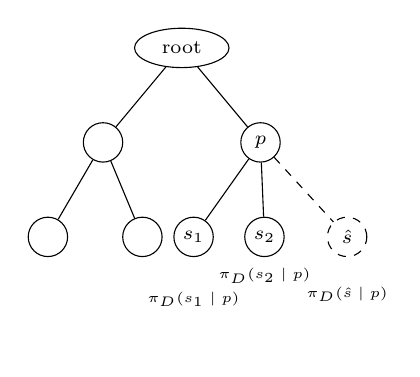
\begin{tikzpicture}[
      every node/.style={
        circle,
        draw,
        minimum size=5mm,
        inner sep=1pt
      },
      virt/.style={
        circle,
        draw,
        dashed,
        minimum size=5mm,
        inner sep=1pt
      }
    ]
      \node[
        ellipse,
        draw,
        minimum width=12mm
      ] (root) {\scriptsize root};

      \node (a) at (-1.0,-1.2) {};
      \node (P) at (1.0,-1.2) {\scriptsize \(p\)};

      \node (a1) at (-1.7,-2.4) {};
      \node (a2) at (-0.5,-2.4) {};

      \node (p1) at (0.15,-2.4) {\scriptsize \(s_1\)};
      \node (p2) at (1.05,-2.4) {\scriptsize \(s_2\)};
      \node[virt] (v) at (2.10,-2.4) {\scriptsize \(\hat{s}\)};

      \draw (root) -- (a);
      \draw (root) -- (P);

      \draw (a) -- (a1);
      \draw (a) -- (a2);

      \draw (P) -- (p1);
      \draw (P) -- (p2);
      \draw[dashed] (P) -- (v);

      \node[draw=none, below=-1mm of p1]
        {\tiny \(\pi_D(s_1\mid p)\)};

      \node[draw=none, below=-4mm of p2]
        {\tiny \(\pi_D(s_2\mid p)\)};

      \node[draw=none, below=-1mm of v]
        {\tiny \(\pi_D(\hat{s}\mid p)\)};
    \end{tikzpicture}
  \end{column}

  \begin{column}{0.60\textwidth}
    \textbf{Virtual-child logit}
\vspace{-0.7em}
    {\scriptsize
    \begin{align*}
      \mu_L(p)
      &=
      \frac{1}{|\mathcal{C}(p)|}
      \sum_{u\in\mathcal{C}(p)} L_D(u),
      \\[0.4em]
      \sigma_L(p)
      &=
      \sqrt{
        \frac{1}{|\mathcal{C}(p)|}
        \sum_{u\in\mathcal{C}(p)}
        \bigl(L_D(u)-\mu_L(p)\bigr)^2
      },
      \\[0.5em]
      L_p(\hat{s})
      &=
      \mu_L(p)+\lambda\,\sigma_L(p).
    \end{align*}
    }
  \end{column}
\end{columns}

\end{frame}


\begin{frame}{Virtual Child \& Parent-Local Prior (cont.)}
\vspace{-2em}
{\color{titledred}\hrule height 1.2pt}
\vspace{0.9em}

Define the available action set $  \mathcal{A}(p)
  =
  \mathcal{C}(p)\cup\{\hat{s}\},$
and assign every action a logit in the same space:
\vspace{0.2em}
{\footnotesize
\begin{equation*}
  L_p(a)
  =
  \begin{cases}
    L_D(a),
      & a\in\mathcal{C}(p),
      \\[0.4em]
    \mu_L(p)+\lambda\sigma_L(p),
      & a=\hat{s}.
  \end{cases}
\end{equation*}

\vspace{0.4em}

\begin{equation*}
  \boxed{
  \pi_D(a\mid p)
  =
  \frac{
    \exp\bigl(L_p(a)/\tau\bigr)
  }{
    \displaystyle
    \sum_{b\in\mathcal{A}(p)}
    \exp\bigl(L_p(b)/\tau\bigr)
  }
  }
\end{equation*}
}

\vspace{0.6em}

\begin{itemize}
  \item Small \(\tau\): concentrates probability on strong actions.
  \item Large \(\tau\): produces a flatter local prior.
\end{itemize}

\end{frame}


\begin{frame}{D-PUCT Selection Procedure}
\vspace{0.1em}
{\color{titledred}\hrule height 1.2pt}
\vspace{1em}

At parent \(p\), each available action
\(a\in\mathcal{A}(p)\) is assigned

{\footnotesize
\begin{equation*}
  \operatorname{D\text{-}PUCT}(p,a)
  =
  V(p,a)
  +
  c\,\pi_D(a\mid p)
  \frac{\sqrt{m_p}}{1+m_{p,a}} .
\end{equation*}
}

\textbf{Selection procedure}

\begin{enumerate}
  \item Start at the root node.
  
  \item At the current node \(p\), select
  \[
    a^\star
    =
    \arg\max_{a\in\mathcal{A}(p)}
    \operatorname{D\text{-}PUCT}(p,a).
  \]

  \item Apply the selected action:
  \begin{itemize}
    \item If \(a^\star\) is a non-leaf real child, move to that child
          and repeat the selection step.
    \item If \(a^\star\) is a leaf child, generate \(k\) children.
    \item If \(a^\star=\hat{s}\), generate one new child of \(p\).
  \end{itemize}
\end{enumerate}

\end{frame}





\HuaweiTitleSlide{Adaptive Memory for Test-Time}{July 22, 2026}











\begin{frame}{Test-Time Learning with Adaptive Memory (EACL'26)}

\begin{columns}[T,onlytextwidth]

\begin{column}{0.63\textwidth}

\begin{itemize}
    \item Maintains an evolving external memory containing useful strategies, insights, and solutions
    \item No parameter updates, ground-truth labels, or human feedback required

    \item \textbf{BL:} solves every problem independently

    \item \textbf{FH:} provides the entire previous history

    \item \textbf{DC-RS:} Their Dynamic-Cheetsheet method. They reused the same LLM to Curate the memory using a different prompt.
\end{itemize}

\vspace{1em}

\[
\text{Retrieve top k previous with output}
\rightarrow
\text{Curate}
\rightarrow
\text{Generate}
\]

\end{column}

\begin{column}{0.4\textwidth}

\centering
\includegraphics[width=0.8\linewidth]{dc_bl.jpg}

\vspace{0.35em}

\includegraphics[width=0.8\linewidth]{dc_fh.jpg}

\vspace{0.35em}

\includegraphics[width=1\linewidth]{dc_rs.jpg}

\end{column}

\end{columns}

\end{frame}






\begin{frame}{Results on AIME}

\begin{columns}[T,onlytextwidth]

\begin{column}{0.58\textwidth}





\begin{itemize}
    \item AIME is a high-school mathematics competition covering algebra, combinatorics, number theory, geometry, and probability
    
\end{itemize}

\vspace{1em}

\begin{center}
\includegraphics[width=0.75\linewidth]{dc_res.jpg}
\end{center}


\end{column}

\begin{column}{0.5\textwidth}

\centering
\includegraphics[width=0.8\linewidth]{ex.jpg}

\end{column}

\end{columns}





\end{frame}



\begin{frame}{{\small ReasoningBank: Scaling Agent Self-Evolving with Reasoning Memory (ICLR'26, Google)}}
\small
Tasks $q_1, \dots, q_N$ arrive in a stream; no ground-truth labels. The agent must evolve using only its own past trajectories and self-verification.
 
\vspace{2pt}
\textbf{Gap in prior literature:} raw trajectories (Synapse) or success-only workflows (AWM)
\begin{itemize}\setlength\itemsep{0pt}
    \item No distillation and mostly raw trajectories only
    \item Failures, a rich source of preventative lessons, are discarded
\end{itemize}
 
\textbf{ReasoningBank:} distills structured memory items from \emph{both} self-judged successful and failed trajectories, forming a closed loop:
(i)~\textbf{retrieval} $\rightarrow$ (ii)~\textbf{extraction} $\rightarrow$ (iii)~\textbf{consolidation} (add)
 
\begin{center}
    \includegraphics[width=0.8\textwidth]{fig_overview.jpg}
\end{center}
\end{frame}


\begin{frame}{How the Memory Is Constructed}
\small
\textbf{Memory item schema} (Markdown, human- and machine-readable):
\begin{itemize}\setlength\itemsep{0em}
    \item \textbf{Title} (strategy identifier)
    \item \textbf{Description} (one sentence)
    \item \textbf{Content} (1--3 sentences of distilled reasoning / pitfalls)
\end{itemize}
  
 
\vspace{3pt}
\textbf{Extraction pipeline (per completed task):}
\begin{enumerate}\setlength\itemsep{1pt}
    \item \textbf{LLM-as-Judge} (same backbone) labels trajectories Success/Failure with no ground truth.
    \item \textbf{Dual prompts}: 
    \begin{itemize}
        \item success $\rightarrow$ explain \emph{why it worked}, extract transferable strategies
        \item failure $\rightarrow$ reflect on the cause, extract preventative lessons.
    \end{itemize}
\end{enumerate}
 
\textbf{Retrieval:} embed the new query, cosine similarity over the pool, take items of the top-$k$ experiences, inject into the system prompt before acting.
\vspace{0.5em}
 
\textbf{Consolidation:} Minimal, new items are simply appended to a pool (no pruning or merging).
\end{frame}


\begin{frame}{MaTTS: Memory-Aware Test-Time Scaling}
\footnotesize
Instead of extracting memory from each rollout independently (a) do it in 
\textbf{MaTTS Parallel} with $k$ rollouts per task to keep consistent patterns and filter spurious ones or
\textbf{MaTTS Sequential} with \emph{self-refinement} within one trajectory that intermediate correction notes become memory signals.

\vspace{-0.3em}

\begin{center}
    \includegraphics[width=0.8\textwidth]{fig_matts.jpg}
\end{center}

\vspace{-1em}

\begin{center}
    \includegraphics[width=0.6\textwidth]{res.jpg}
\end{center}
 

\end{frame}


\begin{frame}{Memory Extractor prompt}

\begin{center}
    \includegraphics[width=1\textwidth]{prompt.jpg}
\end{center}
 
\end{frame}


\begin{frame}{Test-Time Self-Distillation (SDPO), ICLR'26 workshop}
    \textbf{Problem:} With a reward $0$ on every attempt $\rightarrow$ zero advantage, no learning signal until the first solution is found for RLVR (e.g., GRPO).
    
    \vspace{0.5em}
    \textbf{Key idea: the model is its own teacher}
    \begin{itemize}
        \item \emph{Student} $\pi_\theta(y \mid x)$: the model answering cold
        \item \emph{Self-teacher} $\pi_\theta(y \mid x, f)$: the \emph{same weights} re-scoring the failed attempt with environment feedback $f$ (traceback, failing test) in context
        \item With $f$ visible, per-token probabilities shift exactly at the buggy tokens; elsewhere they barely move $\Rightarrow$ dense credit assignment for free
    \end{itemize}
    \vspace{0.5em}
    \textbf{SDPO loop}
    \begin{enumerate}
        \item Sample $G$ attempts, collect feedback
        \item Re-score each attempt under the feedback-augmented prompt
        \item Minimize $\sum_t \mathrm{KL}\big(\pi_\theta(\cdot \mid x, y_{<t}) \,\|\, \mathrm{sg}(\pi_\theta(\cdot \mid x, f, y_{<t}))\big)$
`    \end{enumerate}
\end{frame}

\begin{frame}{Connection to Our Work}
\vspace{-5em}    

SDPO is not a memory mechanism but a way to ensure that, regardless of the RL algorithm we choose, learning occurs from both positive scores and failed attempts.
\vspace{2em}

\textbf{Caveat}: We should not run RL in a stepwise manner. Standard RL updates change the underlying $\pi$, making SDPO inapplicable to the new $\pi$. Instead, SDPO should be integrated directly into whichever RL method we use.






\end{frame}




\HuaweiTitleSlide{Memory-Augmented Search with Failure Feedback}{August 19, 2026}


\begin{frame}{Where Memory Sits in the Loop}
\vspace{0.1em}
\titlerule
\vspace{1.2em}

\begin{center}
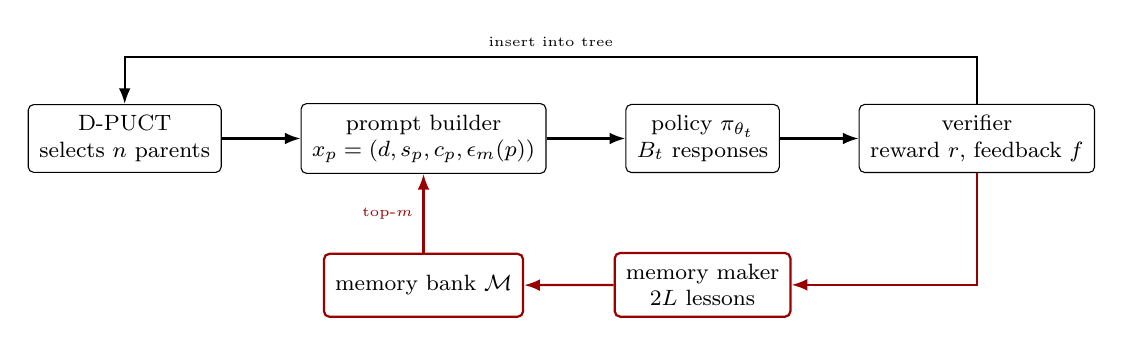
\begin{tikzpicture}[
  node distance=0.6cm,
  box/.style={draw, rounded corners=2pt, minimum height=8mm, align=center,
              font=\footnotesize, inner sep=4pt},
  memnode/.style={box, draw=titledred, thick},
  ar/.style={-{Latex[length=2mm]}, thick}
]
  \node[box] (sel) {D-PUCT\\ selects $n$ parents};
  \node[box, right=1.0cm of sel] (prompt) {prompt builder\\ $x_p=(d,s_p,c_p,\epsilon_m(p))$};
  \node[box, right=1.0cm of prompt] (gen) {policy $\pi_{\theta_t}$\\ $B_t$ responses};
  \node[box, right=1.0cm of gen] (ver) {verifier\\ reward $r$, feedback $f$};

  \node[memnode, below=1.0cm of prompt] (mem) {memory bank $\mathcal{M}$};
  \node[memnode, below=1.0cm of gen] (maker) {memory maker\\ $2L$ lessons};

  \draw[ar] (sel) -- (prompt);
  \draw[ar] (prompt) -- (gen);
  \draw[ar] (gen) -- (ver);
  \draw[ar, titledred] (mem) -- node[left, font=\tiny] {top-$m$} (prompt);
  \draw[ar, titledred] (maker) -- (mem);
  \draw[ar, titledred] (ver.south) |- (maker.east);
  \draw[ar] (ver.north) -- ++(0,0.6) -| node[pos=0.25, above, font=\tiny] {insert into tree} (sel.north);
\end{tikzpicture}
\end{center}

\vspace{0.8em}
\begin{itemize}
  \item Same LLM backbone as the generator, dedicated extraction prompts.
  \item Two calls per step: one over the successes, one over the failures.
\end{itemize}
\end{frame}


\begin{frame}{Version 1}
\vspace{0.1em}
\titlerule
\vspace{1.4em}

Partition step $t$'s responses by verifier reward, subsample each group to $k$,
and send each to the backbone in one call:

\vspace{0.3em}
{\footnotesize
\begin{equation*}
\mathcal{L}_t^{+}=\operatorname{LLM}_{\mathrm{mem}}\bigl(\mathrm{prompt}^{+},\mathcal{S}_t^{(k)},\mathcal{C}_t\bigr),
\qquad
\mathcal{L}_t^{-}=\operatorname{LLM}_{\mathrm{mem}}\bigl(\mathrm{prompt}^{-},\mathcal{F}_t^{(k)},\mathcal{C}_t\bigr)
\end{equation*}
}

\vspace{1.2em}
The bank is additive but deduplicated at entry:

\vspace{0.3em}
{\footnotesize
\begin{equation*}
\mathcal{M}_t=\mathcal{M}_{t-1}\cup\mathcal{D}_\tau\!\left(\mathcal{L}_t^{+}\cup\mathcal{L}_t^{-}\right)
\end{equation*}
}

\vspace{1.2em}
\begin{itemize}
  \item Before expanding a parent $p$, retrieve $m$ lessons by cosine similarity, so all children share one set of lessons.

\end{itemize}
\end{frame}






















\begin{frame}{Experimental Setup}
\vspace{0.1em}
\titlerule
\vspace{1em}

Circle packing, $n=26$. Best known value
$2.635983$. Qwen3-8B with LoRA, $30$ steps of $B_t=512$ rollouts, $8$ parents
$\times$ $64$ children, PUCT.

\vspace{0.8em}
{\small
\begin{center}
\begin{tabular}{lccccccc}
\toprule
Run & Memory & Steps & Rollouts & Best score & Valid & Valid$^{+}$ & Lessons \\
\midrule
\textsc{mem-a}  & yes & 36 & 18{,}432 & 2.635982 & 0.551 & 0.523 & 194 \\
\textsc{mem-b}  & yes & 37 & 18{,}944 & \textbf{2.635983} & 0.734 & 0.709 & 185 \\
\textsc{mem-c}  & yes & 30 & 15{,}360 & 2.515688 & 0.745 & 0.645 & 162 \\
\textsc{no-mem} & no  & 32 & 16{,}384 & 2.525416 & 0.646 & 0.594 & --- \\
\bottomrule
\end{tabular}
\end{center}
}

\vspace{0.8em}
\begin{itemize}
  \item \textsc{mem-a} and \textsc{mem-c} are some configuration differences in A,B, and C.
\end{itemize}
\end{frame}


\begin{frame}{}

\begin{center}
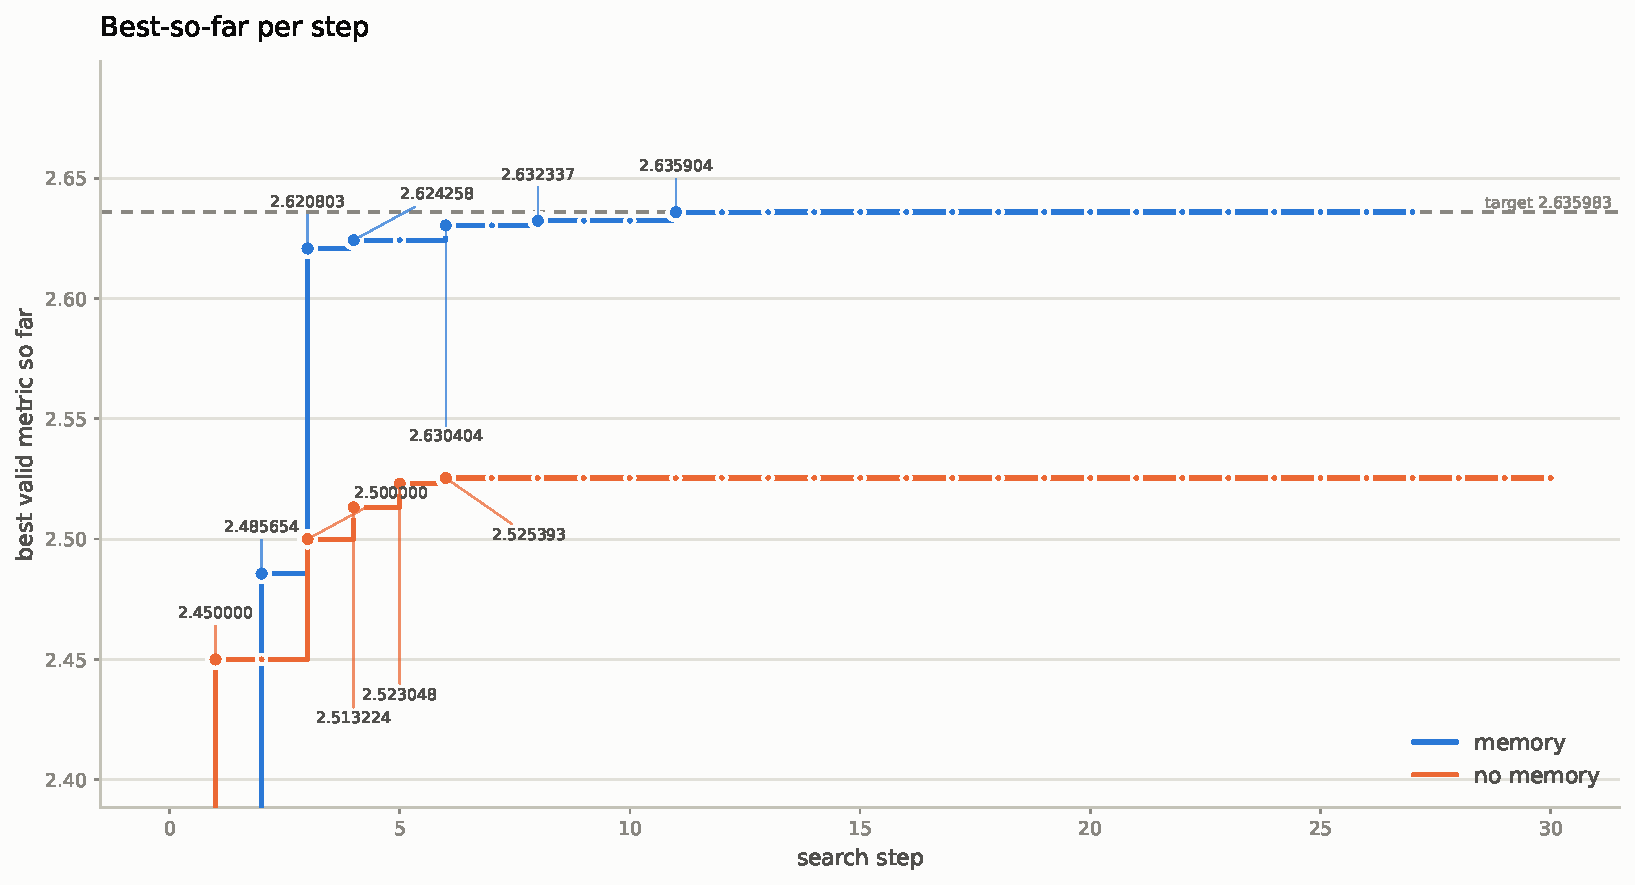
\includegraphics[width=1.05\linewidth]{best_so_far.pdf}
\end{center}


\end{frame}






\begin{frame}{Findings}
\vspace{-3em}
\titlerule
\vspace{1.6em}

\begin{itemize}
  \item $87\%$--$89\%$ of lessons \textbf{never retrieved}; the top five took
        $60\%$--$77\%$ of all retrievals.
  \item Code is $23\%$--$34\%$ of each bank but takes $88\%$--$96\%$ of
        retrieval mass.
  \item All $48$ lessons on global search, ensembles, and restarts:
        \textbf{zero retrievals}. \textsc{mem-b} escaped conditioned only on
        lessons describing the plateau it was leaving.
\end{itemize}

\vspace{1.8em}
\begin{block}{Reason}
The query barely changes across parents, so
the cosine term barely varies
\end{block}
\end{frame}











\begin{frame}{Examples of lessons}
\vspace{-0.4em}
\titlerule
\vspace{0.6em}

{\scriptsize
\setlength{\tabcolsep}{4pt}
\begin{center}
\begin{tabular}{p{0.075\linewidth}p{0.03\linewidth}p{0.115\linewidth}p{0.60\linewidth}}
\toprule
ID & Run & Injected & Lesson text \\
\midrule
\texttt{979e6dc0} & \textsc{c} & 14{,}336 (19.3\%) &
{\ttfamily rows = int(np.ceil(np.sqrt(n)));\newline
x = 0.5 + (col - (cols-1)/2) * (1/(cols-1));\newline
y = 0.5 + (row - (rows-1)/2) * (1/(rows-1));\newline
if row \% 2 == 1: y += np.sqrt(3)/2 / 2} \\
\addlinespace
\texttt{1644ca11} & \textsc{b} & 17{,}600 (19.1\%) &
{\ttfamily dist = np.linalg.norm(centers[i] - centers[j]);\newline
radii[i] = min(radii[i], dist / 2)} \\
\addlinespace
\texttt{d3b941ec} & \textsc{a} & 13{,}888 (15.5\%) &
Clamp circle positions to the unit square bounds: {\ttfamily x = max(min(x,1),0)}. \\
\addlinespace
\texttt{3a29df87} & \textsc{a} & \textbf{0 (0.0\%)} &
Initialize centers with a hexagonal grid layout for $n$ circles, adjusting spacing to fit
the unit square. \\
\bottomrule
\end{tabular}
\end{center}
}

\end{frame}





\begin{frame}{Memory Version 2 --- What a Lesson May Contain}
\vspace{0.1em}
\titlerule
\vspace{1.3em}

\begin{center}
\begin{minipage}{0.86\linewidth}
\begin{block}{}
\centering\large
A lesson may describe an \textbf{operation}. \\
It may never hand over a \textbf{construction}.
\end{block}
\end{minipage}
\end{center}

\vspace{1.3em}
{\small
\begin{center}
\begin{tabular}{lll}
\toprule
\texttt{scope} & Content & Code \\
\midrule
\texttt{local}  & repair, check, diagnostic, guard & up to $4$ lines \\
\texttt{global} & starting configuration, formulation, method family & \textbf{none} \\
\bottomrule
\end{tabular}
\end{center}
}

\vspace{0.6em}
{\small The contrastive call asks why some attempts succeeded \emph{and others
failed}, with each child shown against its parent's score.}
\end{frame}












\begin{frame}{Version 2 --- One Bank, Read and Written}
\vspace{-0.6em}
\titlerule
\vspace{0.5em}

\begin{center}
\resizebox{0.97\linewidth}{!}{
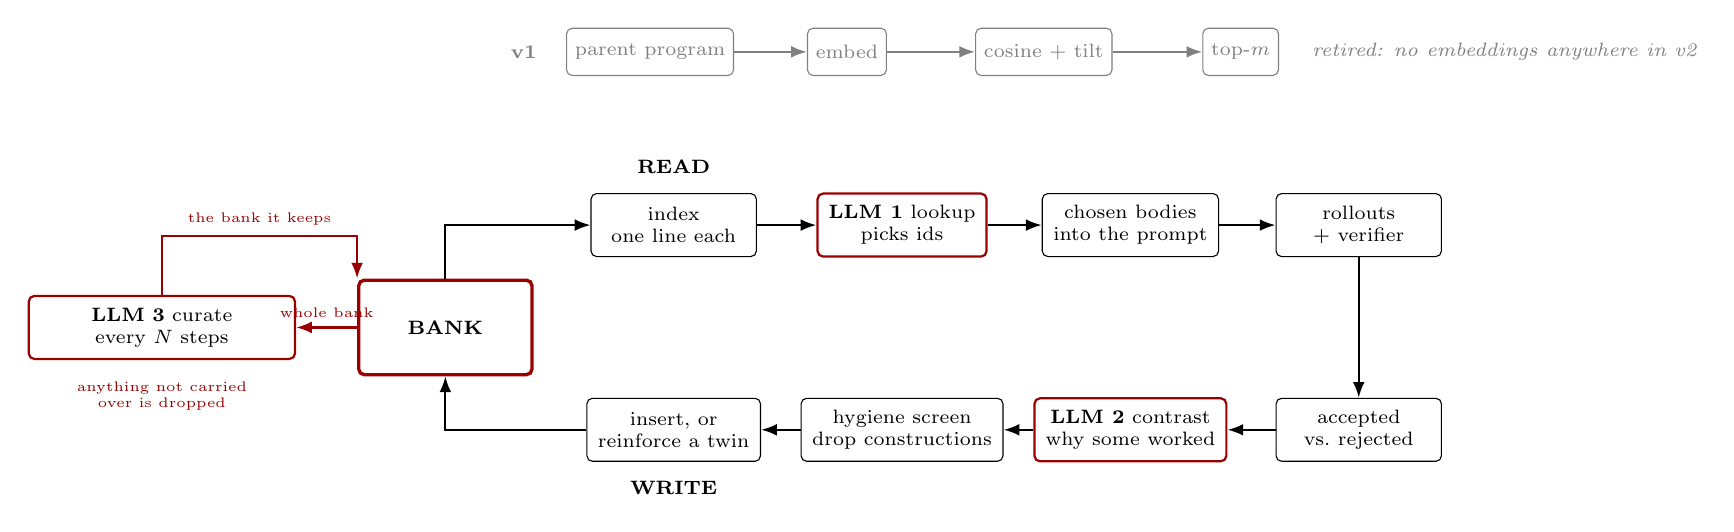
\begin{tikzpicture}[
  box/.style={draw, rounded corners=2pt, align=center, font=\scriptsize,
              inner sep=4pt, minimum height=8mm, minimum width=2.1cm},
  hot/.style={box, draw=titledred, thick},
  bankst/.style={draw=titledred, very thick, rounded corners=2pt, align=center,
                 font=\scriptsize\bfseries, inner sep=5pt,
                 minimum height=12mm, minimum width=2.2cm},
  dead/.style={draw=gray, rounded corners=2pt, align=center, font=\scriptsize,
               inner sep=3pt, minimum height=6mm, text=gray},
  ar/.style={-{Latex[length=2mm]}, thick},
  dar/.style={-{Latex[length=2mm]}, thick, gray},
  lbl/.style={font=\scriptsize\bfseries}
]

  \node[dead]                       (q) at (2.6, 1.9) {parent program};
  \node[dead] (e) at (5.1, 1.9) {embed};
  \node[dead] (c) at (7.6, 1.9) {cosine $+$ tilt};
  \node[dead] (t) at (10.1, 1.9) {top-$m$};
  \node[lbl, text=gray, left=0.25cm of q] {v1};
  \draw[dar] (q) -- (e);  \draw[dar] (e) -- (c);  \draw[dar] (c) -- (t);
  \node[font=\scriptsize\itshape, text=gray, right=0.3cm of t]
       {retired: no embeddings anywhere in v2};

  \node[bankst] (bank) at (0, -1.6) {BANK};

  \node[box] (idx) at (2.9, -0.3) {index\\ one line each};
  \node[hot] (ask) at (5.8, -0.3) {\textbf{LLM 1} lookup\\ picks ids};
  \node[box] (inj) at (8.7, -0.3) {chosen bodies\\ into the prompt};
  \node[box] (rol) at (11.6, -0.3) {rollouts\\ $+$ verifier};
  \node[lbl, above=0.12cm of idx] {READ};

  \draw[ar] (bank.north) |- (idx.west);
  \draw[ar] (idx) -- (ask);
  \draw[ar] (ask) -- (inj);
  \draw[ar] (inj) -- (rol);

  \node[box] (bat) at (11.6, -2.9) {accepted\\ vs.\ rejected};
  \node[hot] (con) at (8.7, -2.9) {\textbf{LLM 2} contrast\\ why some worked};
  \node[box] (scr) at (5.8, -2.9) {hygiene screen\\ drop constructions};
  \node[box] (ins) at (2.9, -2.9) {insert, or\\ reinforce a twin};
  \node[lbl, below=0.12cm of ins] {WRITE};

  \draw[ar] (rol) -- (bat);
  \draw[ar] (bat) -- (con);
  \draw[ar] (con) -- (scr);
  \draw[ar] (scr) -- (ins);
  \draw[ar] (ins.west) -| (bank.south);

  \node[hot, text width=3.1cm] (cur) at (-3.6, -1.6)
       {\textbf{LLM 3} curate\\ every $N$ steps};
  \draw[ar, titledred] (bank.west) -- node[above, font=\tiny] {whole bank} (cur.east);
  \draw[ar, titledred] (cur.north) -- ++(0,0.75)
        -| node[pos=0.25, above, font=\tiny] {the bank it keeps} (bank.north west);
  \node[font=\tiny, text=titledred, align=center, below=0.15cm of cur]
       {anything not carried\\ over is dropped};

\end{tikzpicture}}
\end{center}



\end{frame}





























\begin{frame}{Learning from Failures}
\vspace{-0.6em}
\titlerule
\vspace{0.6em}

{\small A scalar reward says a rollout failed, not \emph{which tokens} caused it.
Failures are $50\%$--$70\%$ of init step's, and constant-reward
groups were skipped entirely. Reuse them as feedback.}

{\footnotesize
\begin{equation*}
  {
  A^{\mathrm{fb}}_{i,\ell}
  =
  \log q_{\bar\theta}\bigl(y_{i,\ell}\mid x_p,f_i,y_{i,<\ell}\bigr)
  -
  \log \pi_{\bar\theta}\bigl(y_{i,\ell}\mid x_p,y_{i,<\ell}\bigr),
  }
  \qquad
  A_{i,\ell}=A^{\mathrm{rew}}_i+\lambda_f(t)\, d_i\, A^{\mathrm{fb}}_{i,\ell}
\end{equation*}
}

\vspace{-0.2em}
\begin{columns}[T,onlytextwidth]
\begin{column}{0.56\textwidth}
{\footnotesize
\begin{itemize}
  \item $q_{\bar\theta}$ is $\pi_{\bar\theta}$ on
        $\mathrm{reprompt}(x_p,f_i)$. 
  \item Positive where the feedback makes the token \emph{more} plausible,
        negative where it makes it less so.
  \item Constant-reward groups become trainable: $A^{\mathrm{rew}}_i=0$ but
        $A^{\mathrm{fb}}$ is not.
\end{itemize}
}
\end{column}

\begin{column}{0.43\textwidth}
\centering
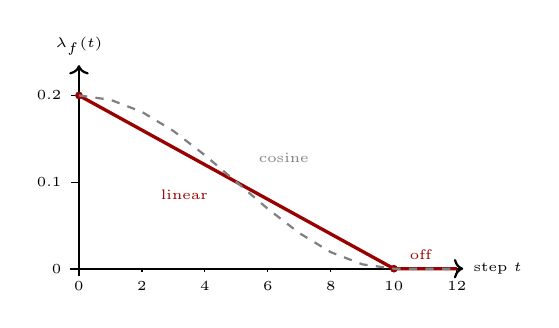
\begin{tikzpicture}[x=0.4cm, y=11cm]
  \draw[->, thick] (-0.3,0) -- (12.2,0) node[right, font=\tiny] {step $t$};
  \draw[->, thick] (0,-0.008) -- (0,0.235) node[above, font=\tiny] {$\lambda_f(t)$};
  \foreach \x in {0,2,4,6,8,10,12}
    \draw (\x,0) -- (\x,-0.004) node[below, font=\tiny] {\x};
  \foreach \y/\l in {0/0, 0.1/0.1, 0.2/0.2}
    \draw (0,\y) -- (-0.25,\y) node[left, font=\tiny] {\l};


  \draw[titledred, very thick] (0,0.2) -- (10,0) -- (12,0);
  \fill[titledred] (0,0.2) circle (1.4pt);
  \fill[titledred] (10,0) circle (1.4pt);
  \node[font=\tiny, titledred, anchor=west] at (10.2,0.016) {off};

  \draw[gray, dashed, thick]
    (0,0.200) -- (1,0.195) -- (2,0.181) -- (3,0.159) -- (4,0.131)
    -- (5,0.100) -- (6,0.069) -- (7,0.041) -- (8,0.019) -- (9,0.005)
    -- (10,0) -- (12,0);
  \node[font=\tiny, gray, anchor=west] at (5.4,0.128) {cosine};
  \node[font=\tiny, titledred, anchor=east] at (4.4,0.086) {linear};
\end{tikzpicture}


\end{column}
\end{columns}

\end{frame}




\begin{frame}{}
\begin{center}
\includegraphics[width=1.05\linewidth]{feedback_vs_baseline.pdf}
\end{center}
    
\end{frame}


\begin{frame}{}
\vspace{-1em}
\begin{center}
\includegraphics[width=1.05\linewidth]{small_variants.pdf}
\end{center}
    
\end{frame}





\HuaweiTitleSlide{Max-Seeking Memory and Adaptive Failure Feedback}{August 26, 2026}







\begin{frame}{Discovery Objective and Notation}
\vspace{-0.35em}
\titlerule
\vspace{0.7em}

\begin{columns}[T,onlytextwidth]
\begin{column}{0.47\textwidth}
\begin{block}{Symbols used in the next slides}
{\footnotesize
\begin{tabular}{@{}cl@{}}
\toprule
$x$ & selected parent program/state \\
$\pi_\theta(\cdot\mid x)$ & current program generator \\
$Y$ & one generated candidate program \\
$R(Y)$ & verified reward (larger is better) \\
$K$ & rollout budget for this parent \\
\bottomrule
\end{tabular}
}
\end{block}
\end{column}

\begin{column}{0.51\textwidth}
\begin{block}{The quantity we want to improve}
\[
Y_1,\ldots,Y_K\sim\pi_\theta(\cdot\mid x),
\]
\vspace{-0.8em}
\[
J_K(\pi_\theta\mid x)
=\mathbb{E}\!\left[\max_{1\le i\le K}R(Y_i)\right].
\]
{\small $J_K$ is the expected reward of the \textbf{best} candidate among the
$K$ attempts.}
\end{block}
\end{column}
\end{columns}

\vspace{0.7em}
\begin{center}
\begin{minipage}{0.86\linewidth}
\begin{block}{Max-seeking, not mean-seeking}
\centering
Improving the typical program is useful only if it does not remove the rare
programs that can produce a new best result.
\end{block}
\end{minipage}
\end{center}
\end{frame}


% \begin{frame}{2. What Is a Proxy, and Why Can It Mislead?}
% \vspace{-0.35em}
% \titlerule
% \vspace{0.55em}

% \begin{block}{Concrete definition}
% A \textbf{proxy} is an easy-to-observe intermediate signal used in place of the
% true objective. Here the true objective is best-of-$K$ reward, but it is sparse,
% noisy, and expensive to estimate repeatedly.
% \end{block}

% \begin{columns}[T,onlytextwidth]
% \begin{column}{0.49\textwidth}
% \begin{block}{Memory proxy}
% Examples are how often a lesson is selected, reused, followed by a valid
% program, or judged consistent with a later solution.

% These signals show that the lesson was \emph{active}; they do not show that it
% raised the best reward relative to no memory.
% \end{block}
% \end{column}
% \begin{column}{0.49\textwidth}
% \begin{block}{Feedback proxy}
% Examples are whether an invalid program was repaired or whether the validity
% rate increased after feedback.

% These signals show that feedback repaired a constraint; they do not show that
% it preserved high-reward directions.
% \end{block}
% \end{column}
% \end{columns}

% \begin{center}
% \color{titledred}\bfseries A useful proxy can improve while the true objective gets worse.
% \end{center}
% \end{frame}


\begin{frame}{Memory Collapse}
\vspace{0.35em}
\titlerule
\vspace{0.55em}

\begin{center}
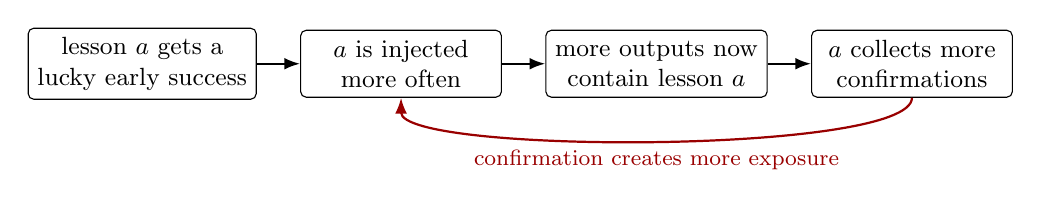
\begin{tikzpicture}[
  box/.style={draw, rounded corners=2pt, align=center, minimum width=2.55cm,
              minimum height=0.85cm, font=\small},
  ar/.style={-{Latex[length=2mm]}, thick}
]
\node[box] (a) {lesson $a$ gets a\\lucky early success};
\node[box, right=0.55cm of a] (b) {$a$ is injected\\more often};
\node[box, right=0.55cm of b] (c) {more outputs now\\contain lesson $a$};
\node[box, right=0.55cm of c] (d) {$a$ collects more\\confirmations};
\draw[ar] (a) -- (b);
\draw[ar] (b) -- (c);
\draw[ar] (c) -- (d);
\draw[ar, titledred] (d.south) .. controls +(0,-0.72) and +(0,-0.72) ..
  node[below, font=\footnotesize, text=titledred] {confirmation creates more exposure} (b.south);
\end{tikzpicture}
\end{center}

\vspace{-0.5em}
\begin{block}{}
Suppose lesson ``$a$'' is injected 20 times and lesson ``$b$'' only 4 times. Even if
the lessons are equally useful, ``$a$'' has many more opportunities to be reused,
confirmed, or followed by a valid output. A count-based score will therefore
favor ``$a$'' partly because the selector already favored ``$a$''.
\end{block}

\begin{block}{What is missing}
For the \emph{same parent} and the \emph{same number of attempts}, would lesson
``$a$'' produce a better maximum than lesson ``$b$'' or no memory?
\end{block}
\end{frame}


\begin{frame}{Memory Collapse}
\vspace{-0.35em}
\titlerule
\vspace{0.2em}

\begin{block}{}
$p_t(m)$ is the probability of injecting lesson $m$ at update $t$;
$u_t(m)$ is its observed proxy score; and $\eta>0$ controls how strongly the
selector reacts to score differences.
\end{block}

\begin{columns}[T,onlytextwidth]
\begin{column}{0.50\textwidth}
\begin{block}{Selection update}
\[
p_{t+1}(m)=
\frac{p_t(m)e^{\eta u_t(m)}}
{\sum_j p_t(j)e^{\eta u_t(j)}}.
\]
% The denominator sums over every lesson $j$.
\end{block}
\end{column}

\begin{column}{0.48\textwidth}
\begin{block}{Compare lessons $a$ and $b$}
\[
\frac{p_{t+1}(a)}{p_{t+1}(b)}
\!=\!\frac{p_t(a)}{p_t(b)}
e^{\eta[u_t(a)-u_t(b)]}.
\]
The exponential multiplies the old selection odds by a factor determined by
the score gap.
\end{block}
\end{column}
\end{columns}

\begin{block}{}
For $\eta=1$ and $u_t(a)-u_t(b)=0.4$, one update multiplies the odds for $a$ by
$e^{0.4}\approx1.49$. If that biased gap lasts for $T=10$ updates, the total
factor is $e^{4}\approx54.6$ without proving that $a$ improves final reward.
\end{block}
\end{frame}


\begin{frame}{Feedback Collapse}
\vspace{-0.35em}
\titlerule
\vspace{0.45em}

\begin{block}{}
For rollout $i$ and token $\ell$,
$A_{i,\ell}=A_i^{\rm rew}+\lambda_f d_iA_{i,\ell}^{\rm fb}.$
\vspace{0.5em}

$A_i^{\rm rew}$ is scientific reward advantage;
$A_{i,\ell}^{\rm fb}$ is the token-level repair signal;
$d_i=1$ only for a failed rollout; and $\lambda_f$ is feedback strength.
\end{block}

\begin{columns}[T,onlytextwidth]
\begin{column}{0.49\textwidth}
\begin{block}{Example: every candidate is invalid}
All candidates receive the same reward, so $A_i^{\rm rew}\approx0$. The
verifier nevertheless gives detailed syntax, timeout, or shape corrections,
so $A_{i,\ell}^{\rm fb}$ remains informative and dense.
\end{block}
\end{column}
\begin{column}{0.49\textwidth}
\begin{block}{What the optimizer then learns}
The update is driven almost entirely by repairs. It favors familiar programs
that are easy to make valid, even if unusual programs are the only route to a
large scientific reward.
\end{block}
\end{column}
\end{columns}

\begin{center}
\color{titledred}\bfseries Repair answers ``is it valid?'', not ``how good can it become?''
\end{center}
\end{frame}


% \begin{frame}{6. Proposal Intuition: Measure What Memory Adds}
% \vspace{-0.35em}
% \titlerule
% \vspace{0.5em}

% \begin{block}{A matched thought experiment}
% Use the same parent $x$ and the same number of attempts $n$ in two arms. The
% only intended difference is whether lesson $m$ is injected.
% \end{block}

% \begin{center}
% \begin{tabular}{lccc}
% \toprule
% Arm & Observed rewards in three attempts & Mean & Best \\
% \midrule
% No memory & $(3,5,7)$ & $5$ & $7$ \\
% With lesson $m$ & $(2,4,11)$ & $5.67$ & $11$ \\
% \bottomrule
% \end{tabular}
% \end{center}

% \vspace{0.65em}
% \begin{columns}[T,onlytextwidth]
% \begin{column}{0.49\textwidth}
% \begin{block}{Marginal value}
% ``Marginal'' means the value added by memory beyond what the no-memory control
% already achieves: here the observed best increases by $11-7=4$.
% \end{block}
% \end{column}
% \begin{column}{0.49\textwidth}
% \begin{block}{Tail value}
% ``Tail'' refers to rare high rewards. We compare the best result because that
% is the part of the distribution relevant to max-seeking discovery.
% \end{block}
% \end{column}
% \end{columns}
% \end{frame}


\begin{frame}{Memory Bandit}
\vspace{0.3em}
\titlerule
% \vspace{0.55em}

% \begin{block}{Best-of-$n$ value with lesson $m$}
\begin{block}{}
\[
M_n(m\mid x)=
\mathbb{E}\!\left[
\max_{1\le j\le n}R(Y_j)
\;\middle|\;x,\;m\text{ is injected}
\right].
\]
generate $n$ candidates from parent $x$, keep the
largest reward, and average that maximum over repeated batches. The symbol
$m=\emptyset$ means no memory.
\end{block}

\begin{block}{Subtract the no-memory counterfactual}
\[
\Delta_m^{(n)}(x)=M_n(m\mid x)-M_n(\emptyset\mid x).
\]
Both terms use the same parent and the same $n$, so the difference isolates the
effect of injecting lesson $m$.
\end{block}

% \begin{columns}[T,onlytextwidth]
% \begin{column}{0.49\textwidth}
% \begin{block}{Why take the maximum?}
% The search returns its best verified candidate. Therefore the value of a batch
% is its largest reward, not its average reward.
% \end{block}
% \end{column}
% \begin{column}{0.49\textwidth}
% \begin{block}{Why take an expectation?}
% Generation is random. Repeating the same $n$-attempt experiment can give a
% different maximum, so $M_n$ averages over that randomness.
% \end{block}
% \end{column}
% \end{columns}
\footnotesize{
\begin{center}
\begin{tabular}{ccl}
$\Delta_m^{(n)}>0$ & $\Rightarrow$ & memory improves the attainable maximum \\
$\Delta_m^{(n)}\approx0$ & $\Rightarrow$ & memory adds no measured value \\
$\Delta_m^{(n)}<0$ & $\Rightarrow$ & memory suppresses better directions
\end{tabular}
\end{center}
}
\end{frame}


% \begin{frame}{8. Then Subtract the No-Memory Control}
% \vspace{-0.35em}
% \titlerule
% \vspace{0.55em}

% \begin{block}{Subtract the no-memory counterfactual}
% \[
% \Delta_m^{(n)}(x)=M_n(m\mid x)-M_n(\emptyset\mid x).
% \]
% Both terms use the same parent and the same $n$, so the difference isolates the
% effect of injecting lesson $m$.
% \end{block}

% \begin{center}
% \begin{tikzpicture}[
%   box/.style={draw, rounded corners=2pt, align=center, minimum width=4.0cm,
%               minimum height=1.05cm, font=\small},
%   ar/.style={-{Latex[length=2mm]}, thick}
% ]
% \node[box] (m) {same parent $x$, same $n$\\inject lesson $m$\\value $M_n(m\mid x)$};
% \node[box, right=1.35cm of m] (z) {same parent $x$, same $n$\\inject no memory\\value $M_n(\emptyset\mid x)$};
% \draw[ar, titledred] (z.south west) .. controls +(-0.4,-0.55) and +(0.4,-0.55) ..
%   node[below, font=\footnotesize, text=titledred] {subtract control from memory} (m.south east);
% \end{tikzpicture}
% \end{center}

% \begin{center}
% \begin{tabular}{ccl}
% $\Delta_m^{(n)}>0$ & $\Rightarrow$ & memory improves the attainable maximum \\
% $\Delta_m^{(n)}\approx0$ & $\Rightarrow$ & memory adds no measured value \\
% $\Delta_m^{(n)}<0$ & $\Rightarrow$ & memory suppresses better directions
% \end{tabular}
% \end{center}
% \end{frame}


\begin{frame}{Memory Bandit}
\vspace{-0.5em}
\titlerule
\vspace{0.5em}

\begin{center}
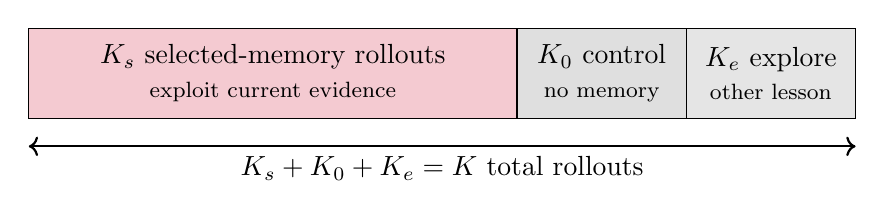
\begin{tikzpicture}[x=1cm,y=1cm]
\draw[fill=huaweired!22] (0,0) rectangle (6.2,1.15);
\draw[fill=bannergray!25] (6.2,0) rectangle (8.35,1.15);
\draw[fill=black!10] (8.35,0) rectangle (10.5,1.15);
\node[align=center] at (3.1,0.58) {$K_s$ selected-memory rollouts\\\footnotesize exploit current evidence};
\node[align=center] at (7.275,0.58) {$K_0$ control\\\footnotesize no memory};
\node[align=center] at (9.425,0.58) {$K_e$ explore\\\footnotesize other lesson};
\draw[<->,thick] (0,-0.35) -- node[below] {$K_s+K_0+K_e=K$ total rollouts} (10.5,-0.35);
\end{tikzpicture}
\end{center}

\vspace{0.65em}
\begin{columns}[T,onlytextwidth]
\begin{column}{0.32\textwidth}
\begin{block}{Selected arm $s$}
Most rollouts may use the currently preferred lesson so useful memory still
accelerates search.
\end{block}
\end{column}
\begin{column}{0.32\textwidth}
\begin{block}{Control arm $0$}
A small permanent no-memory arm estimates what would have happened without
memory.
\end{block}
\end{column}
\begin{column}{0.32\textwidth}
\begin{block}{Exploration arm $e$}
A small permanent exploratory arm tests lessons that are promising or
uncertain.
\end{block}
\end{column}
\end{columns}

% \begin{center}
% \color{titledred}\bfseries The total remains $K$: this is one run, not two full runs.
% \end{center}
\end{frame}




\begin{frame}{Normalize Values}
\vspace{-0.05em}
\titlerule
\vspace{0.35em}

\small

\begin{block}{Raw maxima are unfair}
Even if two arms have the same reward distribution, the maximum of 10 samples
is usually larger than the maximum of 3 samples. This is the
\emph{best-of-more} advantage.
\end{block}

{\small Suppose an arm produced $k$ rewards $\mathbf r=(r_1,\ldots,r_k)$.
To compare it at size $n\le k$, use}
\[
\widehat M_n(\mathbf r)
=
\mathbb{E}_{S}\!\left[
\max_{j\in S}r_j
\right],
\qquad
S\sim\operatorname{Uniform}\{S\subseteq\{1,\ldots,k\}:|S|=n\}.
\]

\begin{columns}[T,onlytextwidth]
\begin{column}{0.52\textwidth}
\begin{block}{Example}
For rewards $(1,2,3)$ and $n=2$, the possible subsets have maxima
$2,3,3$. Therefore
\[
\widehat M_2(1,2,3)=\frac{2+3+3}{3}=\frac{8}{3}.
\]
\end{block}
\end{column}
\begin{column}{0.46\textwidth}
\begin{block}{Matched comparison}
For memory and control arms, set $n=\min(K_m,K_0)$ and compute
\[
\widehat\Delta_m
=\widehat M_n(\mathbf r_m)
-\widehat M_n(\mathbf r_0).
\]
% Here $\mathbf r_m$ and $\mathbf r_0$ are the memory and control reward vectors.
% Both sides are now best-of-$n$.
\end{block}
\end{column}
\end{columns}
\end{frame}

% \begin{frame}{10. Fair Comparison Means Equal Numbers of Chances}
% \vspace{-0.35em}
% \titlerule
% \vspace{0.4em}

% \begin{block}{Start with unequal arm sizes}
% Let $K_m$ be the number of rollouts using lesson $m$, and let $K_0$ be the
% number using no memory. Set
% \[
% n=\min(K_m,K_0).
% \]
% This makes $n$ the largest number of chances that both arms can support.
% \end{block}

% \begin{block}{Convert either arm to best-of-$n$}
% If an arm produced rewards $\mathbf r=(r_1,\ldots,r_k)$ with $k\ge n$, average
% the maximum over uniformly chosen size-$n$ subsets $S$:
% \[
% \widehat M_n(\mathbf r)=
% \mathbb{E}_{S}\!\left[\max_{j\in S}r_j\right],
% \qquad S\subseteq\{1,\ldots,k\},\quad |S|=n.
% \]
% % In plain language: repeatedly pretend that this arm received only $n$ chances,
% % record its best reward, and average those best rewards.
% \end{block}
% \end{frame}


% \begin{frame}{11. Matched Comparison: A Complete Example}
% \vspace{-0.35em}
% \titlerule
% \vspace{0.15em}

% \begin{block}{Observed rewards}
% \[
% \mathbf r_m=(1,4,6,10),\quad K_m=4;
% \qquad
% \mathbf r_0=(3,8),\quad K_0=2.
% \]
% The raw maximum favors memory: $10>8$. But memory received twice as many
% chances, so set $n=\min(4,2)=2$. The matched calculation reverses the result.
% \end{block}

% \begin{columns}[T,onlytextwidth]
% \begin{column}{0.55\textwidth}
% \begin{block}{Memory arm as best-of-2}
% Its six possible pairs have maxima
% \[
% 4,\;6,\;10,\;6,\;10,\;10.
% \]
% Therefore
% \[
% \widehat M_2(\mathbf r_m)=\frac{46}{6}\approx7.67.
% \]
% \end{block}
% \end{column}
% \begin{column}{0.43\textwidth}
% \begin{block}{Control arm as best-of-2}
% It has one pair, with maximum $8$:
% \[
% \widehat M_2(\mathbf r_0)=8.
% \]
% Thus
% \[
% \widehat\Delta_m=7.67-8=-0.33.
% \]
% \end{block}
% \end{column}
% \end{columns}

% \end{frame}


\begin{frame}{Upper confidence bound for memory}
% \vspace{-0.35em}
\titlerule
\vspace{0.45em}

\begin{block}{}
\[
\operatorname{UCB}(m)=
{\overline\Delta_m}
+
{c\,s_R
\sqrt{\frac{\log(1+N)}{1+n_m}}}.
\]
% UCB means \emph{upper confidence bound}: select using an optimistic estimate of
% what the lesson may be worth, not only its current average.
\end{block}

\begin{columns}[T,onlytextwidth]
\begin{column}{0.49\textwidth}
\begin{block}{Measured-value term}
$\overline\Delta_m$ is lesson $m$'s average matched uplift. A reliably positive
lesson remains attractive even after many tests.
\end{block}
\end{column}
\begin{column}{0.49\textwidth}
\begin{block}{Uncertainty term}
$n_m$ is the number of matched tests of $m$; $N=\sum_m n_m$ is all matched
tests. The bonus is large when $n_m$ is small and shrinks as evidence arrives.
\end{block}
\end{column}
\end{columns}

% \begin{center}
% $s_R$ sets reward scale; $c\ge0$ sets the desired amount of exploration.
% \end{center}
\end{frame}


% \begin{frame}{13. UCB: A Numerical Example}
% \vspace{-0.35em}
% \titlerule
% \vspace{0.55em}

% \begin{block}{Two lessons after $N=18$ matched tests}
% For illustration, set $c\,s_R=1$.
% \begin{center}
% \begin{tabular}{lcccc}
% \toprule
% Lesson & mean uplift $\overline\Delta_m$ & tests $n_m$ & uncertainty bonus & UCB \\
% \midrule
% $a$: well tested & $1.00$ & $16$ & $\sqrt{\log(19)/17}\approx0.42$ & $1.42$ \\
% $b$: under-tested & $0.50$ & $2$ & $\sqrt{\log(19)/3}\approx0.99$ & $1.49$ \\
% \bottomrule
% \end{tabular}
% \end{center}
% \end{block}

% \begin{columns}[T,onlytextwidth]
% \begin{column}{0.49\textwidth}
% \begin{block}{Why test lesson $b$?}
% Its measured value is lower, but two tests are not enough to rule out a strong
% lesson. Its uncertainty bonus makes one more test worthwhile.
% \end{block}
% \end{column}
% \begin{column}{0.49\textwidth}
% \begin{block}{What happens afterward?}
% Each new test increases $n_b$, shrinking the bonus. Lesson $b$ must eventually
% show real positive uplift or it will lose priority.
% \end{block}
% \end{column}
% \end{columns}

% \begin{center}
% \color{titledred}\bfseries UCB buys information; it does not declare the uncertain lesson better.
% \end{center}
% \end{frame}


\begin{frame}{Adaptive Feedback}
\vspace{-0.05em}
\titlerule
\vspace{0.45em}

\begin{columns}[T,onlytextwidth]
\begin{column}{0.57\textwidth}
\begin{block}{Validity controller}
Let $v_t$ be the fraction of valid programs at step $t$. Define
\[
\lambda_{\rm eff}(t)=\lambda_{\rm sched}(t)g(v_t),
\]
\[
g(v)=
\begin{cases}
1, & v\le v_{\rm floor},\\[2pt]
\dfrac{v_{\rm target}-v}{v_{\rm target}-v_{\rm floor}},
& v_{\rm floor}<v<v_{\rm target},\\[7pt]
0, & v\ge v_{\rm target}.
\end{cases}
\]
\end{block}
\end{column}

\begin{column}{0.41\textwidth}
\begin{block}{Read it as three regimes}
\begin{itemize}
  \item Below $v_{\rm floor}$: full scheduled feedback.
  \item Between the thresholds: linearly decreasing feedback.
  \item Above $v_{\rm target}$: feedback is off.
\end{itemize}
\end{block}
\begin{block}{Weights}
$\lambda_{\rm sched}(t)$ is the planned weight before gating;
$\lambda_{\rm eff}(t)$ is the weight actually used.
\end{block}
\end{column}
\end{columns}

\vspace{0.5em}
\begin{center}
\color{titledred}\bfseries
Feedback is strong only while invalidity is the bottleneck.
\end{center}
\end{frame}


% \begin{frame}{Adaptive Feedback}
% \vspace{-0.35em}
% \titlerule
% \vspace{0.4em}

% \begin{block}{Magnitude cap}
% Let $F_{i,\ell}=\lambda_{\rm eff}d_iA_{i,\ell}^{\rm fb}$ be the weighted
% feedback term for token $\ell$ of rollout $i$. Rescale it so that
% \[
% \operatorname{mean}_{\ell}|F_{i,\ell}|
% \le
% \rho\max\!\left(|A_i^{\rm rew}|,a_0\right).
% \]
% The left side is the average absolute feedback pressure across tokens.
% $\rho\ge0$ limits it relative to reward; the floor $a_0>0$ still permits repair
% when $A_i^{\rm rew}=0$.
% \end{block}

% \begin{block}{Numerical reading}
% Suppose $|A_i^{\rm rew}|=0.10$, $a_0=0.25$, and $\rho=0.20$. The allowed
% feedback magnitude is
% \[
% 0.20\max(0.10,0.25)=0.05.
% \]
% If the current mean magnitude is $0.40$, multiply the feedback term by
% $0.05/0.40=0.125$. Repair remains possible, but it cannot overwhelm reward.
% \end{block}
% \end{frame}


% \begin{frame}{16. Balance Failure Types and Bound Compute}
% \vspace{-0.35em}
% \titlerule
% \vspace{0.05em}

% \begin{block}{Why random failure sampling can be biased}
% Imagine 100 failures: 80 syntax errors, 10 timeouts, and 10 shape errors. A
% random feedback batch will mostly teach syntax repair, even if timeouts or shape
% errors contain more useful information.
% \end{block}

% \begin{columns}[T,onlytextwidth]
% \begin{column}{0.52\textwidth}
% \begin{block}{Two explicit limits}
% Let $\mathcal B_{\rm fb}$ be failures sent to the teacher and
% $\mathcal B_{{\rm fb},e}$ those sharing normalized error signature $e$:
% \[
% |\mathcal B_{\rm fb}|\le B,
% \qquad
% |\mathcal B_{{\rm fb},e}|\le C.
% \]
% $B$ caps total teacher calls; $C$ prevents one error type from filling the
% batch.
% \end{block}
% \end{column}
% \begin{column}{0.46\textwidth}
% \begin{block}{Illustrative balanced batch}
% With $B=30$ and $C=10$, the example can contribute at most 10 syntax, 10
% timeout, and 10 shape failures---instead of roughly 24, 3, and 3.
% \end{block}
% \begin{block}{Compute switch}
% If $\lambda_{\rm eff}=0$, generate no teacher feedback. Once validity is high,
% both feedback pressure and its compute cost disappear.
% \end{block}
% \end{column}
% \end{columns}
% \end{frame}


\begin{frame}{Results}
\vspace{-2.35em}
\titlerule
\vspace{0.35em}

\begin{center}
\footnotesize
using Qwen8B- Seed 42 \;|\; 12 steps \;|\; 64 rollouts/step \;|\; 768 rollouts/run (SOTA: 0.380876 using 50 step, 512/step, gpt-120B)
\end{center}

\vspace{0.05em}
\begin{center}
\footnotesize
\renewcommand{\arraystretch}{1.22}
\begin{tabular}{lcccc}
\toprule
Arm & Best $C_5\downarrow$ & Valid overall & Valid at step 11 & Distinct constructions \\
\midrule
Plain & 0.381327 & 48.0\% & 84.4\% & 175/369 \;(47\%) \\
Memory only & \color{titledred}\bfseries 0.381264$^{\dagger}$
            & 41.5\% & 51.6\% & \color{titledred}\bfseries 274/319 \;(86\%) \\
Feedback only & \color{blue!70!black}\bfseries 0.381289
                       & 59.5\% & 90.6\% & 222/457 \;(49\%) \\
Memory + feedback & \color{titledred}\bfseries 0.381116 & 56.3\%
                  & \color{titledred}\bfseries 90.6\% & 150/432 \;(35\%) \\
\bottomrule
\end{tabular}
\end{center}

\vspace{0.35em}
{\scriptsize $^{\dagger}$Best rollout; the archive kept a worse
duplicate-program execution. Memory + feedback values use its first 12 steps
(through step 11); the full 22-step run reached $C_5=0.381115477$ at step 19.}

% \vspace{0.5em}
% \begin{columns}[T,onlytextwidth]
% \begin{column}{0.49\textwidth}
% {\color{blue!70!black}\large\bfseries feedback works}\par
% \small It beats plain on the best score while raising overall validity by
% 11.5 percentage points.
% \end{column}
% \begin{column}{0.49\textwidth}
% {\color{green!45!black}\large\bfseries Both wins reliability}\par
% \small 93.8\% final-step validity, but a weaker extreme solution than plain or
% memory-only.
% \end{column}
% \end{columns}

% \vspace{0.45em}
% {\scriptsize Feedback-only uses $B_{\rm fb}=16$ and
% $C_{\rm signature}=4$; the other rows retain their original settings.
% $^{\dagger}$Best rollout; the archive kept a worse duplicate-program execution.
% Target: $C_5=0.380876$.}
\end{frame}



\begin{frame}{}
\vspace{-0.15em}
% \titlerule
\vspace{0.15em}

\begin{columns}[T,onlytextwidth]
\begin{column}{1\textwidth}
\centering
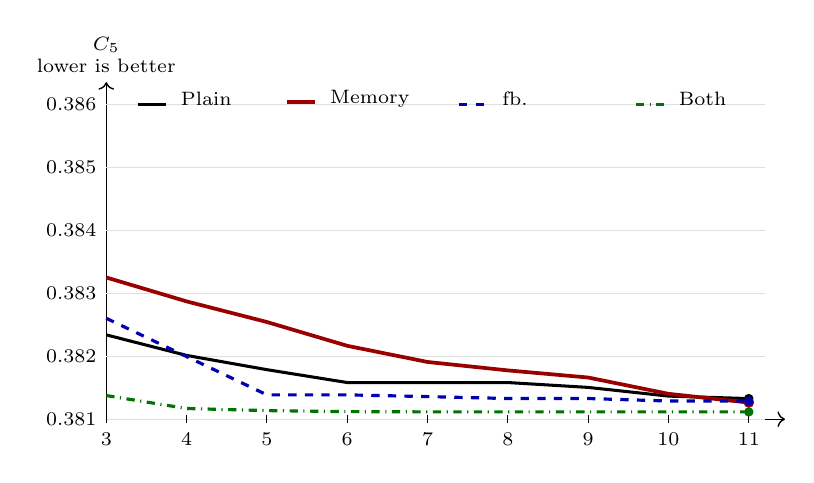
\begin{tikzpicture}[x=1.02cm,y=0.80cm]
  % Axes and grid.  The vertical coordinate is 1000(C5 - 0.381).
  \draw[->,line width=0.5pt] (0,0) -- (8.45,0);
  \draw[->,line width=0.5pt] (0,0) -- (0,5.35)
    node[above,font=\scriptsize,align=center] {$C_5$\\lower is better};
  \foreach \yy/\lab in {0/0.381,1/0.382,2/0.383,3/0.384,4/0.385,5/0.386}{
    \draw[gray!25] (0,\yy) -- (8.2,\yy);
    \node[left,font=\scriptsize] at (0,\yy) {\lab};
  }
  \foreach \xx/\lab in {0/3,1/4,2/5,3/6,4/7,5/8,6/9,7/10,8/11}{
    \draw (\xx,0.06) -- (\xx,-0.06);
    \node[below,font=\scriptsize] at (\xx,-0.06) {\lab};
  }

  \draw[black,line width=1.1pt]
    plot coordinates {(0,1.338741) (1,1.012422) (2,0.786228)
      (3,0.581799) (4,0.581799) (5,0.581799) (6,0.504634)
      (7,0.366687) (8,0.327465)};
  \draw[titledred,line width=1.35pt]
    plot coordinates {(0,2.249836) (1,1.870235) (2,1.542608)
      (3,1.164993) (4,0.908481) (5,0.774578) (6,0.661509)
      (7,0.402814) (8,0.263858)};
  \draw[blue!70!black,dashed,line width=1.15pt]
    plot coordinates {(0,1.601299) (1,0.994326) (2,0.386264)
      (3,0.386264) (4,0.358635) (5,0.328259) (6,0.328259)
      (7,0.288672) (8,0.288672)};
  \draw[green!45!black,dash dot,line width=1.15pt]
    plot coordinates {(0,0.375258) (1,0.169773) (2,0.136500)
      (3,0.120505) (4,0.116046) (5,0.116020) (6,0.115941)
      (7,0.115764) (8,0.115764)};

  \fill[black] (8,0.327465) circle (1.7pt);
  \fill[titledred] (8,0.263858) circle (1.9pt);
  \fill[blue!70!black] (8,0.288672) circle (1.7pt);
  \fill[green!45!black] (8,0.115764) circle (1.7pt);

  \node[anchor=west,font=\scriptsize] at (0.25,5.08) {
    \tikz\draw[black,line width=1.1pt] (0,0)--(0.35,0);\; Plain};
  \node[anchor=west,font=\scriptsize] at (2.10,5.08) {
    \tikz\draw[titledred,line width=1.35pt] (0,0)--(0.35,0);\; Memory};
  \node[anchor=west,font=\scriptsize] at (4.25,5.08) {
    \tikz\draw[blue!70!black,dashed,line width=1.15pt] (0,0)--(0.35,0);\; fb.};
  \node[anchor=west,font=\scriptsize] at (6.45,5.08) {
    \tikz\draw[green!45!black,dash dot,line width=1.15pt] (0,0)--(0.35,0);\; Both};
\end{tikzpicture}

{\scriptsize Cumulative best valid score; steps 0--2 omitted for late-stage resolution.}
\end{column}

% \begin{column}{0.30\textwidth}
% {\color{blue!70!black}\large\bfseries Feedback recovers}\par
% \small With the $16/4$ cap, feedback reaches $0.381386$ at step 5 and
% $0.381289$ at step 10.

% \vspace{0.65em}
% {\color{titledred}\large\bfseries Late: memory}\par
% \small Memory-only lags early, then reaches the best observed tail,
% $0.381264$, at step 11.

% \vspace{0.65em}
% {\color{green!45!black}\large\bfseries Equal budgets}\par
% \small The comparison fixes rollout count; it does not establish convergence.
% \end{column}
\end{columns}



\end{frame}



\begin{frame}{Erdos math: Feedback at step 11}
    
\includegraphics[width=\linewidth]{erdos_solution.pdf}
\end{frame}




\begin{frame}{Next step: adaptive rollout allocation}
\vspace{0.15em}
\titlerule
\vspace{1em}

\begin{columns}[T,onlytextwidth]
\begin{column}{0.8\textwidth}
\centering

\includegraphics[width=\linewidth]{search_tree.pdf}

% \vspace{-0.25em}
% {\scriptsize Fixed expansion creates wide 16-child fans; most children are
% evaluated once and never become parents.}
\end{column}

\begin{column}{0.23\textwidth}
\footnotesize
\begin{block}{What the tree reveals}
Among 399 eligible pre-final children, only 39 (9.8\%) were expanded later.
% Fixed $4\times16$ allocation gives only four informed choices per 64 rollouts.
\end{block}

\begin{block}{Budgeted D-PUCT}
Use microbatches of $b$. After each one, choose
\textsc{Open}$(p)$ (new sibling) or \textsc{Descend}$(p,c)$ (continue branch).
% \[
% \begin{aligned}
% \widehat{\operatorname{EI}}_b(a)
% &=\widehat{\mathbb E}\!\left[
%   \left(\max_{j\le b}R_j(a)-r_t^\star\right)_+
% \right],\\[-1pt]
% S_t(a)&=\widehat{\operatorname{EI}}_b(a)+\beta_tU_t(a).
% \end{aligned}
% \]
\end{block}

% Progressive widening limits breadth:
% $|\mathcal C(p)|\le kN(p)^\alpha$, $0<\alpha<1$. Total compute stays at 64.
\end{column}
\end{columns}
\end{frame}


\end{document}
